% -*- TeX -*- -*- FR -*-
\documentclass[francais,letterpaper]{uds-article}

%-----------------------------------------------------------------------------
%----- Identification des packages n�cessaires
%-----------------------------------------------------------------------------

\usepackage{babel}
\usepackage{color}
\usepackage[latin1]{inputenc}
%\usepackage{udstitle,dfd}
%\newcommand{\diamant}{Diamant}
\setlength{\oddsidemargin}{0.25in}
\setlength{\evensidemargin}{0.25in}
\setlength{\textwidth}{6.0in}
%\setlength{\parskip}{0.2in}
\newcounter{auxcounter}
\renewcommand{\baselinestretch}{1.5}
\setlength{\parskip}{1.5ex plus0.5ex minus0ex}

\newcommand{\ints}{\renewcommand{\baselinestretch}{1.0}\small \normalsize}
\newcommand{\intm}{\renewcommand{\baselinestretch}{1.5}\small \normalsize}
\newcommand{\intd}{\renewcommand{\baselinestretch}{2.0}\small \normalsize}
\newcommand{\todo}[1]{\textcolor[rgb]{1.00,0.00,0.00}{(TODO: #1)}}

\newcommand{\bi}{\begin{itemize}}
\newcommand{\ei}{\end{itemize}}
\newcommand{\be}{\begin{enumerate}}
\newcommand{\ee}{\end{enumerate}}
\newcommand{\bd}{\begin{description}}
\newcommand{\ed}{\end{description}}



\newcommand{\bv}{\verb}

\newcommand{\bve}{\verb*}

\newcommand{\brun}{\noindent $\triangleright$}
\newcommand{\erun}{$\triangleleft$}

\newcommand{\ang}{\textsf}
\newcommand{\key}{\textsf}
\newcommand{\ita}{\textit}
\newcommand{\bld}{\textbf}
\newcommand{\dos}{\textsc}
\newcommand{\pro}{\texttt}

\newcommand{\diamant}{DIAMANT}
\newcommand{\dia}{DIAMANT 1.0}
\newcommand{\dx}{DIAMANT 1.6}
\newcommand{\saphir}{SAPHIR}
\newcommand{\sig}{SIG}

%% commandes pour les corrections du document
\usepackage{color}
\usepackage{ulem}
\newcommand{\corrpascal}[1]{\textcolor[rgb]{0,0,1}{(Pascal: #1)}}
\newcommand{\corryannick}[1]{\textcolor[rgb]{1.00,0.00,0.00}{(Yannick: #1)}} 


%-----------------------------------------------------------------------------
%----- Page Titre
%-----------------------------------------------------------------------------

\Titre{\textbf{-Projet \dx{}-} \\ \\
SOFTWARE DESIGN DOCUMENT \\
\small{\emph{IEEE SDD standard 1016-1998}}\\
}
\Logo{Images/logoDiamantNew.eps}
\Auteurs{Yannick Syam}
\Date{\today}

%-----------------------------------------------------------------------------
%----- Identification des fichiers des pages pr�liminaires et bibliographique
%-----------------------------------------------------------------------------

\FichierResume{}
\FichierRemerciements{}
\FichierGlossaire{} % \FichierLexique est �quivalent
\FichiersBibliographie{udsplain}{}

%-----------------------------------------------------------------------------
%----- Le document
%-----------------------------------------------------------------------------

\includeonly{SDD/intro,SDD/decomposition,SDD/dependency,SDD/interface,SDD/detailled}

\begin{document}
\begin{articleDX}

%\chapter{Description de la structure de donn�es de \diamant{}}

Le noeud principal de la structure de donn�es de \diamant{} est repr�sent� par la classe \emph{LoadData} (voir figure \ref{datastruct}). Cette classe contient la liste des diff�rentes ressources, � savoir:

\begin{itemize}
    \item \emph{StudentsList} (voir figure \ref{datastruct}): elle repr�sente la structure de donn�es contenant la liste des �tudiants.\\
    \item \emph{RoomsList} (voir figure \ref{datastruct}): elle repr�sente la structure de donn�es contenant la liste des locaux.\\
    \item \emph{InstructorsList} (voir figure \ref{datastruct}): elle repr�sente la structure de donn�es contenant la liste d'instructeurs.\\
    \item \emph{ActivitiesList} (voir figure \ref{datastruct}): elle repr�sente la structure de donn�es contenant la liste d'activit�s.\\
\end{itemize}

Chacune des listes de ressources cit�es ci-dessus h�rite de la super classe \emph{ResourceList}. \emph{ResourceList} contient la liste de tous les �l�ments d'une ressource. Cette liste d'�l�ments est en r�alit� une liste d'objects de type \emph{Resource}. L'object \emph{Resource} d�crit quand � lui un �l�ment par sa cl� (\emph{resourceKey}), son identifiant (\emph{resourceID}) et la nature de cet object (\emph{resourceObject}). Il est � noter que \emph{resourceObject} peut �tre de type \emph{Instructor} ou \emph{Activity} ou \emph{Room} ou encore \emph{Student}

Nous d�crirons chacune des structures dans les prochaines sections.

\begin{figure}[h]
  % Requires \usepackage{graphicx}
  \begin{center}
    \includegraphics[width=430pt]{Images/loaddata.eps}
    \caption{Structure de donn�es}\label{datastruct}
  \end{center}
\end{figure}


\section{\emph{LoadData}}
Cette classe est charg�e de la gestion de deux taches principales
:
\begin{enumerate}
    \item \textbf{Le chargement de fichiers} :  Dans cette �tape, l'int�grit� des fichier des ressources est d'abord v�rifi�e et ensuite chaque fichier est charg� dans un vecteur de bytes pour leur post�rieur
    traitement. Cette t�che est effectu� � l'aide de la classe \emph{FilterFile} de la librairie
    \emph{com.iLib.gIO.FilterFile}.
    \item \textbf{La cr�ation des listes de ressources} : Dans cette �tape chaque liste de ressources est cr��e et peupl�e
    (remplie) avec les �l�ments correspondantes. Cette t�che est
    effectu�e en utilisant les classe d�crites � continuation.
\end{enumerate}

\section{\emph{ResourceList}}
Cette classe impl�mente la structure de donn�es
\emph{ResourceList}.  Elle d�clare les m�thodes
\emph{analyseTokens()} et \emph{buildResourceList()} qui
permettent de peupler la liste du ressource. Cette classe d�finie
les m�thodes n�cessaires pour ins�rer, �liminer, �diter, chercher
et trier les ressources.

\section{\emph{***List}}
Cet ensemble repr�sente les classes \emph{RoomsList},
\emph{InstructorsList}, \emph{ActivitiesList},
\emph{StudentsList}.  Ces classes h�ritent de la super classe
\emph{ResourceList} et, par cons�quent, elles impl�mentent les
m�thodes \emph{analyseTokens()} et \emph{buildResourceList()}.

Comme un cas sp�cial, la classe \emph{StudentsList} a son propre
impl�mentation des m�thodes \emph{removeStudent} et
\emph{removeStudent} car dans ce cas, il faut valider l'existence
de courses de choix de l'�tudiant avant d'ins�rer un nouveau
ressource � la liste et l'existence . \textbf{(V�rifier cette
phrase avec Yannick, pour quoi removeStudent??)}.

\section{\emph{Resource}}
Cette classe impl�mente la structure de donn�es \emph{Resource}.
Elle d�finie les m�thodes n�cessaires pour ins�rer, �diter et
obtenir les champs de la ressource.

\section{\emph{Instructor}}
Cette classe repr�sente la disponibilit� d'un instructeur
appartenant au fichier d'instructeurs (Voir section 1.2). Elle
impl�mente les m�thodes pour g�rer (ins�rer, �liminer, �diter,
obtenir) la disponibilit� d'un instructeur.

\section{\emph{Room}}
Cette classe repr�sente l'information d'un local appartenant au
fichier de locaux (Voir section 1.4).  Elle impl�mente les
m�thodes pour g�rer (ins�rer, �liminer, �diter, obtenir) les
diff�rents propri�t�s d'un local, cela inclut sa disponibilit�.

\section{\emph{Student}}
Cette classe repr�sente l'information d'un �tudiant appartenant au
fichier d'�tudiants (Voir section 1.1).  Elle impl�mente les
m�thodes pour g�rer (ins�rer, �liminer, �diter, obtenir) les
diff�rents propri�t�s d'un �tudiant, cela inclut se choix de
cours.

\section{\emph{Activity}}
Cette classe repr�sente l'information d'une activit� appartenant
au fichier d'activit�s (Voir section 1.3).  Elle impl�mente les
m�thodes pour g�rer (ins�rer, �liminer, �diter, obtenir) les
diff�rents propri�t�s d'une activit�, cela inclut ....\textbf(�
finir)


\part{Architecture}
\chapter{Introduction}


    \section{But}

    \diamant{} est un logiciel servant � la construction d'horaires de
    cours et d'examens sur plusieurs sites � partir d'une interface
    utilisateur.

    \section{Conventions propres � ce document}

    Les anglicismes devront �tre en italique.

    \section{Auditoire cibl� et suggestions de lecture}

    Ce document s'adresse � toutes les personnes impliqu�es dans le
    d�veloppement de \diamant{} tout au long de son cycle de vie: il
    s'agit des utilisateurs, des analystes, des architectes, des
    concepteurs, des testeurs et du chef de projet.

    \section{�tendu du projet}

    \diamant{} est un logiciel de construction d'horaires pr�sent� aux
    utilisateurs sous forme de fen�tre avec une barre de menus,
    contenant des sous-menus. La fen�tre principale pr�sente une
    grille d�crivant l'horaire sur lequel l'utilisateur travaille. En
    dessous de la grille horaire se trouve une barre de t�ches
    \corrpascal{Est-ce une barre de ``t�che'' ou une barre de
    ``statut'' ?}  montrant les ressources en utilisation (�tudiants,
    enseignants, activit�s et locaux) et les conflits d�tect�s.

    Les sous-menus sont de deux types~: ceux qui d�clenchent
    l'ex�cution d'une fonctionnalit� et ceux qui appellent une bo�te
    de dialogue, puis d�clenchent des actions. En g�n�ral ces menus
    entra�nent une mise � jour des donn�es en fonction du traitement
    d�clench�.


    \section{R�f�rences}

    Manuel d'utilisation de \diamant{}. 
\chapter{Description de la d�composition}

Pour fonctionner, le logiciel \dx{} a besoin de la machine virtuelle
Java. Pour construire un horaire \dx{} a besoin d'un ensemble de
fichiers. Le d�ploiement de \dx{} devrait donc se faire en consid�rant
les deux autres entit�s dont il a besoin (voir figure
\ref{datastruct}).

\begin{figure*}[h]
  % Requires \usepackage{graphicx}
  \begin{center}
    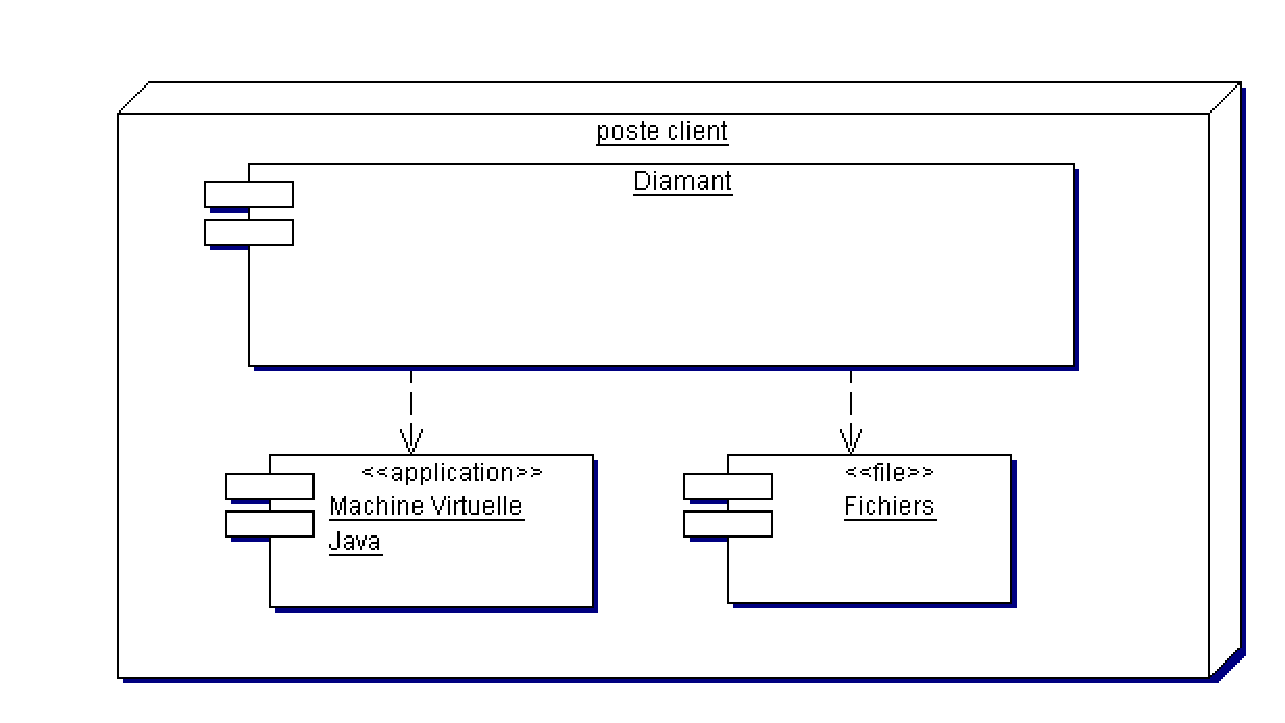
\includegraphics[width=350pt]{SDD/images/Deploiement-global.eps}
    \caption{Syst�me \dx{}}\label{datastruct}
  \end{center}
\end{figure*}


\section{Description des fichiers d'entr�e de  \diamant{}}

\dx{} utilisent les fichiers suivants~:

\begin{enumerate}
    \item �tudiants
    \item Instructeurs
    \item Activit�s
    \item Locaux
\end{enumerate}

Les trois premiers sont produits au STI (Syst�me informatique central)
et transf�r�s via FTP.  Le fichier de locaux est produit localement
par l'utilisateur.

Tous les fichiers ont un format rigide. Le nombre de caract�res et
leur position est � respecter obligatoirement.

Les indexes de cha�nes de caract�res commencent � \verb!0!.

    \subsection{Fichier d'�tudiants}\label{student}

    Ce fichier est un h�ritage du format \saphir{}.

        \subsubsection{Exemple des donn�es qu'il contient}

        \begin{verbatim}
001342
009008132035030720003LUPIEN MY05
CTB301101 GIS251102 GIS351102 GRH111101 GRH332101
009011991290000520021AUDET FRE05
CTB341101 FEC111102 FEC444101 GIS114101 MAR221107
009022232035010720003AUDET STE05
CTB443102 CTB451101 CTB513101 CTB563101 CTB613102
009027042035010720003VEILLEUX 05
CTB443101 CTB451102 CTB513102 CTB563101 CTB613102
009031242035010720003FAUCHER M05
        \end{verbatim}

        \subsubsection{Signification des donn�es}

        Il existe trois types de lignes :

        \begin{enumerate}
            \item nombre d'�tudiants dans le fichier;
            \item identification de l'�tudiant et nombre de cours
                  qu'il prend;
            \item l'identification de cours que l'�tudiant suit.
        \end{enumerate}

        La structure du fichier :

        \begin{enumerate}
            \item La cha�ne du d�but du fichier $n$, \verb!001342!,
                  nous indique le nombre d'�tudiants contenus dans ce
                  fichier. Il s'agit d'une ligne du premier type.
            \item Ensuite il y a $n$ couples de lignes du type 2 et 3.

            \begin{enumerate} 
                \item La ligne de type 2 contient des chiffres et des
                      lettres correspondant au num�ro d'identification
                      unique de l'�tudiant, son nom et le nombre de
                      cours qu'il suit.
                \item La ligne de type 3 contient les cours et
                      �ventuellement les groupes
            \end{enumerate}
        \end{enumerate}

        Les d�tails de la ligne de type 2.

\begin{itemize}
    \item Le matricule de l'�tudiant correspond aux huit premiers
          caract�res du num�ro d'identification (Indices 0 � 7).  Dans
          notre exemple, \verb!00900813! pour l'�tudiant \verb!LUPIEN!
          et \verb!00901199! pour l'�tudiante \verb!AUDET!.
    \item Le programme auquel l'�tudiant appartient correspond ensuite
          aux six caract�res suivants.  Soit \verb!203503! dans le cas
          du premier �tudiant (Indices 8 � 13).
    \item L'instance du programme que l'�tudiant suit correspond aux
          deux caract�res suivants.  Soit \verb!07! dans le cas du
          premier �tudiant (Indices 14 � 15).
    \item Des informations sur l'admission de l'�tudiant sont donn�es
          par les cinq caract�res suivants.  Les quatre premiers
          correspondent � l'ann�e d'admission tandis que le cinqui�me
          indique le trimestre d'admission.  Soit \verb!20003! dans le
          cas du premier �tudiant (Indices 16 � 20).
    \item Suivent ensuite neuf caract�res pour indiquer le nom de
          famille de l'�tudiant suivi d'un espace et de son pr�nom
          (coup� apr�s neuf espaces) (Indices 21 � 29).  Soit, dans
          notre exemple, \verb!LUPIEN MY! dans le cas du premier
          �tudiant.  Dans certains cas le nom prend les neuf
          caract�res.
    \item Vient alors un chiffre de deux caract�res qui correspond en
          fait au nombre de cours que suit l'�tudiant.  \verb!05! dans
          le cas du premier �tudiant (Indices 30 � 31).
\end{itemize}

Les d�tails de la ligne de type 3.

Elle contient la liste des activit�s suivies par l'�tudiant s�par�es
par un espace. Voici un exemple d'information correspondant � chaque
cours.

\begin{itemize}
    \item Soit \verb!CTB301101! dans le cas du premier �tudiant.  Les
          6 premiers caract�res (\verb!GEI441!) \corrpascal{GEI441 sort de o�?  On vient de parler de CTB301...} correspondent au
          num�ro du cours. Le septi�me caract�re (\verb!1!) correspond
          � la nature ou type d'activit� du cours (1=Le�on Magistrale
          et 2=autre). Les 2 derniers caract�res (\verb!01!) sont
          facultatifs dans un fichier et ils correspondent au groupe
          d'activit� dans lequel l'�tudiant est assign�.
\end{itemize}

Un fichier peut avoir le groupe d'activit� pour certains �tudiants,
Facult� d'administration. \corrpascal{Je ne comprends pas le sens de cette phrase (elle ne se termine pas bien)}

        \subsubsection{D�finition  et utilisation des champs}

        \corrpascal{On vient de faire un saut quantique.  On parle de quoi ici?  Le lecteur n'a plus de r�f�rence, de contexte.  Il semble que l'on parle de champs dans une classe...}

        \pro{long int eMatricule} correspond aux indices 0 � 7 de la
        ligne de type deux.  Il est mis dans \verb!_resourceKey!.

        \pro{String eNom} correspond aux indices 21 � 29 de la ligne
        de type deux.  Il est mis dans \verb!_resourceID!.

        \pro{String eAuxField} correspond aux indices 8 � 20 de la
        ligne de type deux.  Il est mis dans \verb!_auxField!.

        \pro{String eSelectedCourse} il peut avoir 1 � $n$
        \pro{eSelectedCourse}, qui sont consid�r�s comme une liste \corrpascal{Il ne faut pas m�langer design et sp�cification.  On pourrait tr�s bien utiliser une autre SD qu'une liste} de
        cours, ceci correspond aux cours dans la ligne de type trois.
        Il est mis dans \verb!_resourceAttach!.

    \subsection{Fichier d'instructeurs}\label{instructor}

Ce fichier contient les donn�es de disponibilit�s des enseignants.
Ce fichier est aussi un h�ritage du format \saphir{}.

\subsubsection{Exemple des donn�es qu'il contient}


\begin{verbatim}
116
ATALLA, NOUREDDINE
1 1 1 1 5 5 5 5 5 5 5 5 5 5
5 5 5 5 5 5 5 5 5 5 5 5 5 5
5 5 5 5 5 5 5 5 5 5 5 5 5 5
5 5 5 5 5 5 5 5 5 5 5 5 5 5
1 1 1 1 5 5 5 5 5 5 5 5 5 5
BALLIVY, G�RARD
1 1 1 1 5 1 1 1 1 1 5 5 5 5
1 1 1 1 5 1 1 1 1 1 5 5 5 5
1 1 1 1 5 1 1 1 1 1 5 5 5 5
1 1 1 5 5 1 1 1 1 5 5 5 5 5
1 1 1 1 5 1 1 1 5 5 5 5 5 5
\end{verbatim}


\subsubsection{Signification des donn�es}

Il existe trois types de lignes :

\begin{enumerate}
    \item le nombre d'enseignants dans le fichier;
    \item l'identification de l'enseignant;
    \item disponibilit� d'une journ�e.
\end{enumerate}

La structure du fichier :

\begin{enumerate}
    \item La cha�ne du d�but du fichier $n$, \verb!116!, nous indique
          le nombre d'enseignants contenus dans ce fichier. Il s'agit
          d'une ligne du premier type.
    \item Ensuite il y a $n$ couples de lignes une de type 2 et cinq de type 3.
    \begin{enumerate}
        \item La ligne de type 2 est une cha�ne de caract�res
              correspondant nom et pr�nom de l'enseignant. La cha�ne
              ne doit pas exc�der trente caract�res.
        \item La ligne de type 3 d�crit la disponibilit� de
              l'enseignant sur une journ�e et comporte quatorze
              entiers s�par�s par un espace.
    \end{enumerate}
\end{enumerate}

Les d�tails de la ligne de type 3.

Elle contient la liste des disponibilit�s d'un enseignant sur une
journ�e et comporte quatorze entiers (0 ou 1) \corrpascal{pourtant
dans l'exemple c'est 1 ou 5} s�par�s par un espace.

Chacune des cinq lignes de type 3 repr�sente une journ�e, en
commen�ant par lundi, jusqu'� vendredi. Chaque colonne correspondant �
un entier (0 ou 1) repr�sente une heure dans la journ�e (8h30, 9h30,
10h30, 11h30, 12h30, 13h30, 14h30, 15h30, 16h30, 17h30, 18h30, 19h00,
20h00 et 21h00). Les disponibilit�s sont ainsi connues entre 8h30 et
21h00.

\subsubsection{D�finition  et utilisation des champs}

\pro{String eNom} correspond aux nom et pr�nom de la ligne de type
deux.  Il est mis dans \verb!_resourceID!.

\pro{String eVailability} \corrpascal{Vailability?} correspond � la
liste des disponibilit�s des lignes de type trois.  elle est mise dans
\verb!_resourceAttach!.

\subsection{Fichier d'activit�s}\label{activity}

Ce fichier contient des informations concernant les cours offerts �
une session. Nous y retrouvons la liste des activit�s associ�es,
l'agencement du cours, le nom de l'enseignant qui le donnera, etc.
C'est un fichier pr�alable � la construction de l'horaire.

\subsubsection{Exemple des donn�es qu'il contient}


\begin{verbatim}

ADM1111  A
1
1
LUC LAJOIE


 2
 2 1
 2 1 4 2
1 1
C1-387 C1-380
0 0
0 0
0 0

ADM1111  B
1
1
R�AL CAOUETTE


 1
 3
 2 12
1
C1-387
0
0
0

AMC6401  A
1
1
FADI AL-HAMED


 2
 2 1
 2 1 4 2
1
D73020
0
0
0
\end{verbatim}


\subsubsection{Signification des donn�es}

Il existe treize types de lignes :

\begin{enumerate}
    \item la ligne vide;
    \item l'identification du cours;
    \item l'�tat du cours (actif ou inactif);
    \item le nombre d'activit�s associ�es au cours;
    \item le nom de l'enseignant du cours;
    \item le nombre d'unit�s de p�riodes s�par�es (exp: une unit� de 2h et une autre de 1h);
    \item la dur�e de chacune des unit�s pr�vues � la ligne pr�c�dente;
    \item le jour et l'heure de d�but de chacune des unit�s d�crites � la ligne pr�c�dente;
    \item l'�tat du local affect� � chaque unit� (fix� ou non fix�);
    \item le nom du local assign� � chaque unit�;
    \item le type de locaux requis � chaque unit�;
    \item le type de locaux requis � chaque unit�;
    \item �tat d'affectation de chaque unit� dans la grille horaire.
\end{enumerate}

La structure du fichier :


\begin{enumerate}
    \item Le fichier commence par une ligne vide, il s'agit d'une
          ligne du premier type.
    \item Ensuite il y a $n$ couples de lignes allant du type 2 au
          type 13.
    \begin{enumerate}
        \item La ligne de type 2 est une cha�ne de caract�res
              correspondant au sigle du cours (\verb!ADM1111 A!).
              Ceci d�crit la le�on magistrale \verb!1!  du cours
              \verb!ADM111! avec le groupe \verb!A!).  Dans l'exemple
              cette ligne contient \verb!ADM1111 A!
        \item La ligne de type 3 d�crit l'�tat du cours, c'est une
              valeur enti�re (0 si le cours est inactif et 1 dans
              l'autre cas).  Dans l'exemple cette ligne contient
              \verb!1!
        \item La ligne de type 4 d�crit le nombre d'activit�s
              associ�es au cours, c'est une valeur enti�re.  Dans
              l'exemple cette ligne contient \verb!1!
        \item La ligne de type 5 est une cha�ne de caract�res
              correspondant au nom de l'enseignant.  Dans l'exemple
              cette ligne contient \verb!LUC LAJOIE!
        \item La ligne de type 6 le nombre de blocs de p�riodes
              s�par�es de la premi�re fiche (ex: si nous avons deux
              heures de cours coll�es � trois endroits diff�rents dans
              l'horaire, l'entier sera 3).  Dans l'exemple cette ligne
              contient \verb!2!
        \item La ligne de type 7. Nous avons une suite de nombres qui
              correspond � la dur�e de chacun des blocs pr�vus � la
              ligne pr�c�dente.  Dans ce cas-ci, la dur�e du premier
              bloc est de deux p�riodes alors que la dur�e du deuxi�me
              est de seulement une p�riode.  Dans l'exemple cette
              ligne contient \verb!2 1!
        \item La ligne de type 8, On a une liste d'entiers
              repr�sentant le jour et l'heure de chacun des blocs
              pr�c�dents.  Par exemple, \texttt{2 1} nous indique que
              le premier bloc a lieu le mardi � 8h30 alors que
              \texttt{4 2} nous apprends que le deuxi�me bloc est le
              jeudi � 9h30.  Dans le exemple cette ligne contient
              \verb!2 1 4 2!
        \item La ligne de type 9.  Cette ligne nous indique si le
              local de cette activit� est fix� ou non.  Effectivement,
              un \texttt{1} nous dit qu'il l'est alors qu'un
              \texttt{0} nous indique le contraire.  Dans l'exemple
              cette ligne contient \verb!1 1!
        \item La ligne de type 10. Sur cette ligne, nous avons les nom
              des locaux pour le premier et le deuxi�me bloc
              respectivement.  Dans l'exemple cette ligne contient
              \verb!C1-387 C1-380!
        \item La ligne de type 11. Puis vient le type de locaux requis
              par cette activit� (voir le manuel d'utilisation de
              \saphir{} \cite{ruben94}).  Dans l'exemple cette ligne
              contient \verb!0 0!
        \item La ligne de type 12. Idem (voir le manuel d'utilisation
              de \saphir{} \cite{ruben94}).  Dans l'exemple cette
              ligne contient \verb!0 0!
        \item La ligne de type 13. Finalement, cette rang�e permet de
              savoir si le bloc � �t� pr�-affect� � l'horaire
              \texttt{(1)} ou non \texttt{(0)}.  Dans le'exemple cette
              ligne contient \verb!0 0!
    \end{enumerate}
\end{enumerate}

Ensuite le fichier continue.

\subsection{Fichier de locaux}\label{room}

\subsubsection{Exemple des donn�es qu'il contient}

\begin{verbatim}
//Facult� des sciences;

//Nom du local;Capacit�;Fonction;Liste des caract�ristiques;Notes;

D13012;32;211;08,11,14,57;laboratoire de chimie;
D13013;40;211;08,11,57;laboratoire de chimie;
D13014;20;211;08,44,57;laboratoire de chimie;
D13016;18;211;08,57;laboratoire de chimie;
\end{verbatim}

\subsubsection{Signification des donn�es}

\begin{description}
    \item[Premi�re ligne] cette ligne repr�sente la facult�.
    \item[Deuxi�me ligne] cette ligne d�crit le fichier.
    \item[Troisi�me ligne] cette ligne est blanche.
    \item[Quatri�me ligne] cette ligne d�crit l'organisation des
         informations sur les locaux.
    \item[Cinqui�me ligne] cette ligne est blanche \corrpascal{Elle ne
         l'est pas dans l'exemple}
    \item[De la sixi�me � la derni�re ligne ] chaque ligne donne les
         informations sur un local. Chaque information est s�par�e par
         un \texttt{';'} et est d�crite comme suit:
    \begin{itemize}
        \item Le nom du local \texttt{D13012} pour le premier local.
        \item La capacit� du local \texttt{32} pour le premier local.
        \item La fonction du local \texttt{211} pour le premier local
              (voir le manuel d'utilisation de \saphir{} \cite{anoyme94})
        \item Liste des caract�ristiques 08,11,14,57 pour le premier
              local (voir le manuel d'utilisation de \saphir{}
              \cite{anoyme94}). Il peut y avoir plusieurs
              caract�ristique, elles seront s�par�es par des
              \texttt{','}
        \item La description du local; \texttt{laboratoire de chimie}
              pour le premier local.
    \end{itemize}
\end{description}


\section{D�composition modulaire (Mod�le Objet)} \label{module}

\subsection{Choix du mod�le}

\subsubsection{Contexte}
    L'objectif de la majorit� des syst�mes informatiques est de
    r�cup�rer les donn�es d'un entrep�t de donn�es (fichiers, base de
    donn�es) et de les pr�senter � l'utilisateur. \corrpascal{c'est une g�n�ralisation ``dangeureuse''} Une fois que
    l'utilisateur a modifi� les donn�es, le syst�me stocke les mises �
    jour dans l'entrep�t. Comme le principal flux d'informations
    s'effectue entre l'entrep�t de donn�es et l'interface utilisateur,
    nous pourrions �tre tent� de lier ces deux �l�ments afin de
    r�duire le volume de code et am�liorer les performances de
    l'application.

    Cette approche qui peut nous para�tre naturelle n'est pas sans
    pr�senter certains probl�mes non n�gligeables. L'un d'eux est que
    l'interface utilisateur a tendance � changer plus fr�quemment que
    le syst�me de stockage des donn�es. Autre probl�me du couplage des
    donn�es avec les �l�ments d'interface utilisateur, les
    applications m�tier \corrpascal{sans explication de ce qu'est une
    application ``m�tier'', c'est m�langeant} tendent � int�grer une
    logique m�tier qui va bien au-del� de la transmission de donn�es.

\subsubsection{Probl�me}

Comment rendre modulaire l'interface utilisateur d'une application de
sorte que chaque partie puisse �tre ais�ment modifi�e
individuellement?

\subsubsection{Facteurs � prendre en compte}

Les facteurs suivants agissent sur le syst�me dans le contexte pr�sent
et doivent �tre pris en compte dans la recherche de la solution au
probl�me :

\begin{itemize}
    \item La logique d'interface utilisateur est modifi�e plus
          fr�quemment que la logique m�tier. Il est possible, par
          exemple, d'ajouter de nouvelles fen�tres d'interface ou de
          r�organiser les fen�tres existantes. Si le code de
          pr�sentation et la logique m�tier sont associ�s dans un seul
          et m�me objet, vous devrez modifier l'objet contenant la
          logique m�tier chaque fois que vous souhaiterez changer
          l'interface utilisateur. Cette d�marche risque d'introduire
          des erreurs et n�cessite � chaque modification de
          l'interface, m�me minime, de tester de nouveau l'ensemble de
          la logique m�tier.\\
    \item Dans certains cas, l'application affiche les m�mes donn�es
          sous plusieurs formes. Par exemple, un analyste pr�f�rera
          visualiser les donn�es dans une feuille de calcul alors que
          ses managers choisiront les graphiques � secteur pour
          afficher les m�mes donn�es. Certaines interfaces utilisateur
          clientes riches pr�sentent simultan�ment plusieurs vues des
          m�mes donn�es. Si l'utilisateur modifie les donn�es dans une
          vue, le syst�me doit automatiquement mettre � jour toutes
          les autres vues.\\
    \item La conception d'interfaces visuellement efficaces et
          attirantes n�cessite g�n�ralement des comp�tences autres que
          celles requises pour le d�veloppement d'une logique m�tier
          complexe. Il est bien rare qu'une m�me personne pr�sente
          cette double comp�tence. Il est donc pr�f�rable de s�parer
          l'effort de d�veloppement de ces deux parties.\\
    \item L'activit� de l'interface utilisateur se compose
          g�n�ralement de deux �l�ments : la pr�sentation et la mise �
          jour. La partie pr�sentation r�cup�re les donn�es d'un
          entrep�t de donn�es et les met en forme avant de les
          afficher. Lorsque l'utilisateur effectue une action sur les
          donn�es, la partie mise � jour passe la main � la logique
          m�tier pour mettre � jour les donn�es.\\
    \item Le code de l'interface utilisateur d�pend g�n�ralement plus
          de la machine que la logique m�tier. Si vous souhaitez faire
          migrer l'application d'une application monolithique � une
          application sur navigateur ou � une application sur
          assistant personnel ou sur t�l�phone mobile compatible Web,
          vous devez r��crire une bonne partie du code de l'interface
          utilisateur alors que la logique m�tier pourra rester
          inchang�e. Une s�paration claire de ces deux �l�ments permet
          d'acc�l�rer la migration et de r�duire le risque
          d'introduction d'erreurs dans la logique m�tier.\\
    \item La cr�ation de tests automatis�s pour les interfaces
          utilisateur est g�n�ralement plus longue et difficile que
          les m�mes tests pour la logique m�tier. On comprend donc que
          r�duire le couplage du module de code m�tier et du module de
          l'interface utilisateur permet d'am�liorer les capacit�s
          d'�valuation de l'application.
\end{itemize}

\subsubsection{Solution}

\dx{} est une application GUI\footnote{Graphical User Interface}. Sa
construction requiert donc l'utilisation d'un mod�le adapt�: le mod�le
Model-View-Controller (MVC), car il s�pare la mod�lisation du domaine,
la pr�sentation et les actions reposant sur l'entr�e utilisateur en
trois composant distincts :



\begin{figure*}[h]
  % Requires \usepackage{graphicx}
  \begin{center}
    \includegraphics[width=350pt]{SDD/images/Deploiement-diamant.eps}
    \caption{Architecture MVC de \dx{}}\label{datastruct}
  \end{center}
\end{figure*}

\begin{description}
    \item[Le mod�le:] il g�re le comportement et les donn�es
         sp�cifiques de \dx{} (les enseignants, les locaux, les cours,
         les �tudiants, la grille horaire, etc), r�pond aux demandes
         d'informations sur son �tat (souvent issues de la vue) ainsi
         qu'aux instructions de changement d'�tat (souvent issues du
         contr�leur).
    \item[La vue:] elle offre un ensemble fen�tre, dialogue, menu, etc
         permettant une mise en page de l'affichage d'informations. Il
         permet � l'utilisateur de faire des requ�tes sur le mod�le et
         de visualiser les r�sultats.
    \item[Le contr�leur:] il g�re les �v�nements d'entr�e de
         l'utilisateur � partir de la souris ou du clavier. Chaque vue
         a un contr�leur associ� qui la connecte avec avec les
         p�riph�rique d'entr�e.
\end{description}

\subsection{Description du mod�le}

Le mod�le de \dx{} est b�ti autour de cinq principaux sous-composants:
la structure composite (SetOfXxx) permettant de g�rer des collections
de donn�es, le sous-composant \verb!Model!, le sous-composant
\verb!Data!, le sous-composant \verb!TTStructure! et enfin le
sous-composant \verb!Optimization! (voir figure \ref{model}).

\begin{figure*}[h]
  % Requires \usepackage{graphicx}
  \begin{center}
    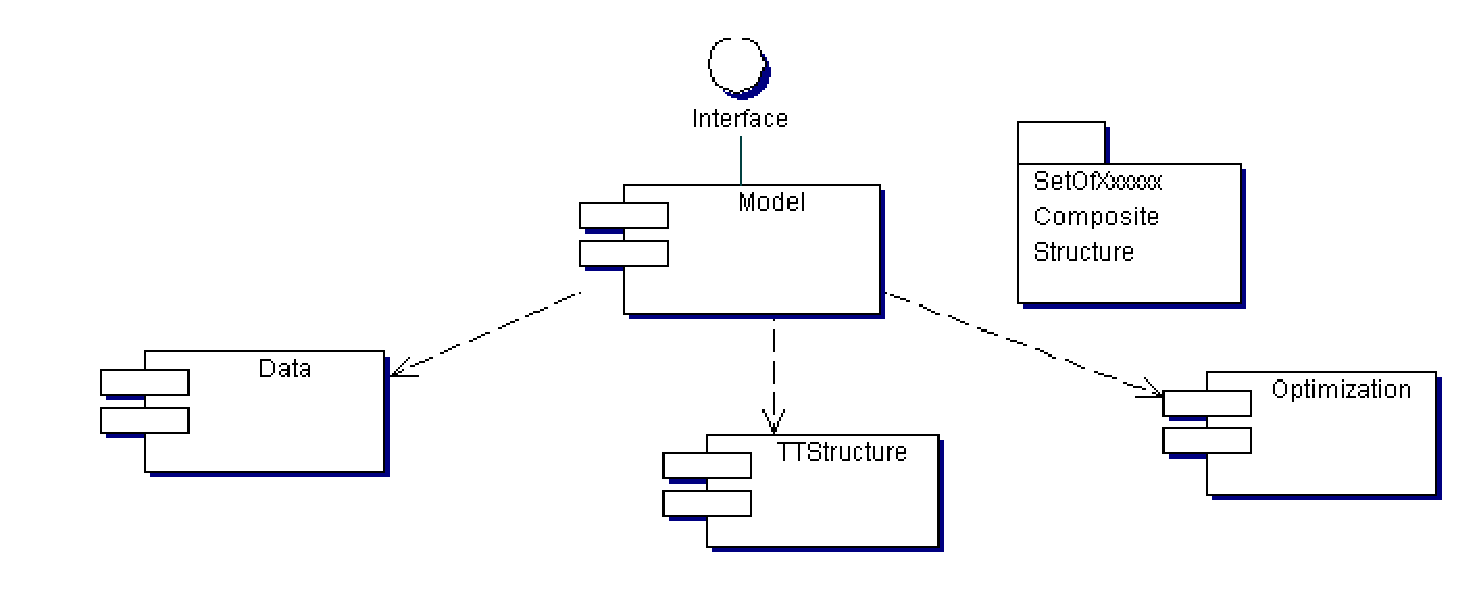
\includegraphics[width=350pt]{SDD/images/Component-Global.eps}
    \caption{Architecture du composant mod�le de \dx{}}\label{model}
  \end{center}
\end{figure*}

\subsubsection{Description de la structure composite SetOfXxx}

Cette structure s'inspire du pattern composite et elle permet
d'organiser les donn�es dans un arbre (voir figure \ref{composite})
\corrpascal{la figure \ref{composite} n'a rien � voir avec un
arbre}. Une structure composite contient plusieurs objets (dans notre
cas, ces objets sont de m�me type), chaque objet est compos� de
plusieurs champs, les champs peuvent �tre de types de donn�es
diff�rents.

Afin de pouvoir manipuler indiff�remment les structures composites �
partir de n'importe quel champ, nous les avons pourvu de certains
comportement (inspir�s des principales commandes SQL des bases de
donn�es relationnelles):

\begin{itemize}
    \item interroger (getXxx),
    \item manipuler des entr�es (setXxx, insertXxxx, removeXxx),
    \item d�finir des donn�es (addXxx)
\end{itemize}


\begin{figure*}[h]
  % Requires \usepackage{graphicx}
  \begin{center}
    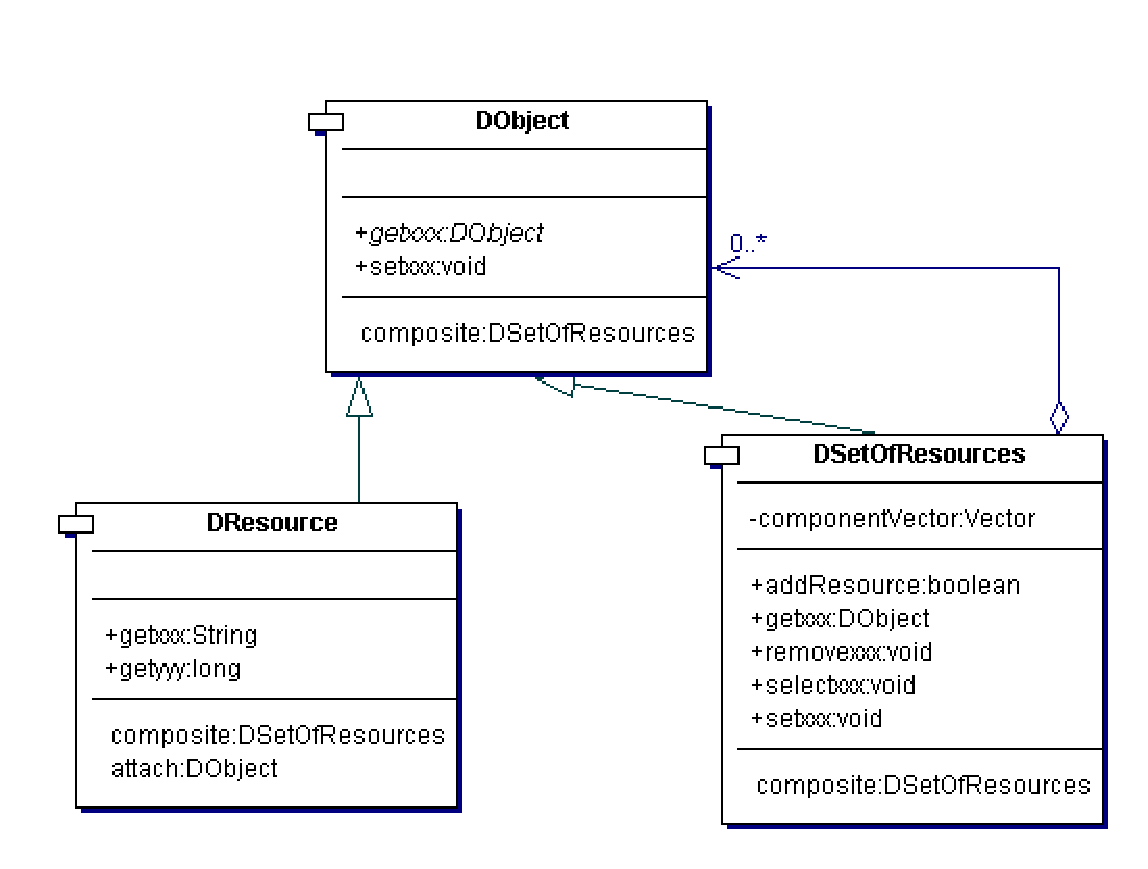
\includegraphics[width=300pt]{SDD/images/Composite_Structure.eps}
    \caption{Description de la structure composite SetOfXxx}\label{composite}
  \end{center}
\end{figure*}

\subsubsection{Description du sous-composant model}

Le sous-composant \verb!model! repr�sente le point d'entr�e du
composant mod�le (de l'architecture MVC). Il est l'interface � travers
laquelle le mod�le communique avec les autres composants que sont la
vue et le contr�leur.  Il impl�mente donc uniquement les m�thodes
utiles � la vue et au contr�leur.

\corrpascal{les explications sur les sous-mod�les mod�le-structure et processus est pour le moins ambigue}

La conception du sous-composant \verb!model! est faite de sorte �
l'organiser autour de trois entit�s: l'entit� model, l'entit�
structure et l'entit� comportement ou processus (voir figure
\ref{submodel}).

\begin{figure*}[h]
  % Requires \usepackage{graphicx}
  \begin{center}
    \includegraphics[width=350pt]{SDD/images/sub_component_model.eps}
    \caption{Description du sous-composant model}\label{submodel}
  \end{center}
\end{figure*}

\begin{description}
    \item[L'entit� structure: ] elle fournit les interfaces permettant
    d'acc�der aux donn�es (�tudiants, instructeurs, locaux, activit�s
    et grille horaire).
    \item[L'entit� process: ] elle fournit les interfaces permettant
    de lancer les op�rations sur les donn�es (cr�ation des �v�nements,
    algorithmes, etc).
    \item[L'entit� model: ] elle regroupe les interfaces offertes par
    l'entit� structure et l'entit� process.
\end{description}

Vue le nombre d'interfaces qu'il pourrait avoir entre l'entit�
structure et l'entit� model, vue la redondance de ces interfaces dans
l'entit� model, il est paru n�cessaire de r�organiser ces entit�s et
de les faire passer de trois � deux. Ainsi le sous-composant model
sera r�organis� autour de deux entit�s: l'entit� model-structure et
l'entit� process.

\begin{description}
    \item[L'entit� process: ] elle fournit les interfaces permettant
    de lancer les op�rations sur les donn�es (cr�ation des �v�nements,
    algorithmes, etc).
    \item[L'entit� model-structure: ] elle regroupe les interfaces
    offertes par l'entit� process en plus de celles permettant
    d'acc�der aux donn�es.
\end{description}

\subsubsection{Description du sous-composant data}

Le sous-composant data (voir figure \ref{subdata}) permet tout d'abord
de g�rer les acc�s aux donn�es physiques (lecture et �criture).  Il
permet ensuite d'organiser les donn�es sous une forme pr�d�finie
(structure de donn�es). Il permet enfin de manipuler ces donn�es
(ajout, suppression, modification, recherche, tri). Les donn�es
manipul�es ici sont les enseignants, les locaux, les �tudiants et les
activit�s.

\begin{figure*}[h]
  % Requires \usepackage{graphicx}
  \begin{center}
    \includegraphics[width=350pt]{SDD/images/sub_component_data.eps}
    \caption{Description du sous-composant data}\label{subdata}
  \end{center}
\end{figure*}

\subsubsection{Description du sous-composant ttstructure}

Le sous-composant \verb!TTstructure! permet de d�crire et manipuler la
grille horaire. La structure de ce sous-composant est de type
hi�rarchique et le noeud principal est appel� timetable (voir figure
\ref{struct}). Une timetable peut �tre compos�e d'un ou de plusieurs
cycle(s). Un cycle peut �tre compos� d'un ou de plusieurs jour(s). Un
jour peut �tre compos� d'une ou de plusieurs s�quence(s). Une s�quence
peut �tre compos�e d'une ou de plusieurs p�riode(s). La p�riode est la
plus petite unit� d'une timetable, elle est d�crite en minutes.

 \begin{figure*}[h]
  % Requires \usepackage{graphicx}
  \begin{center}
    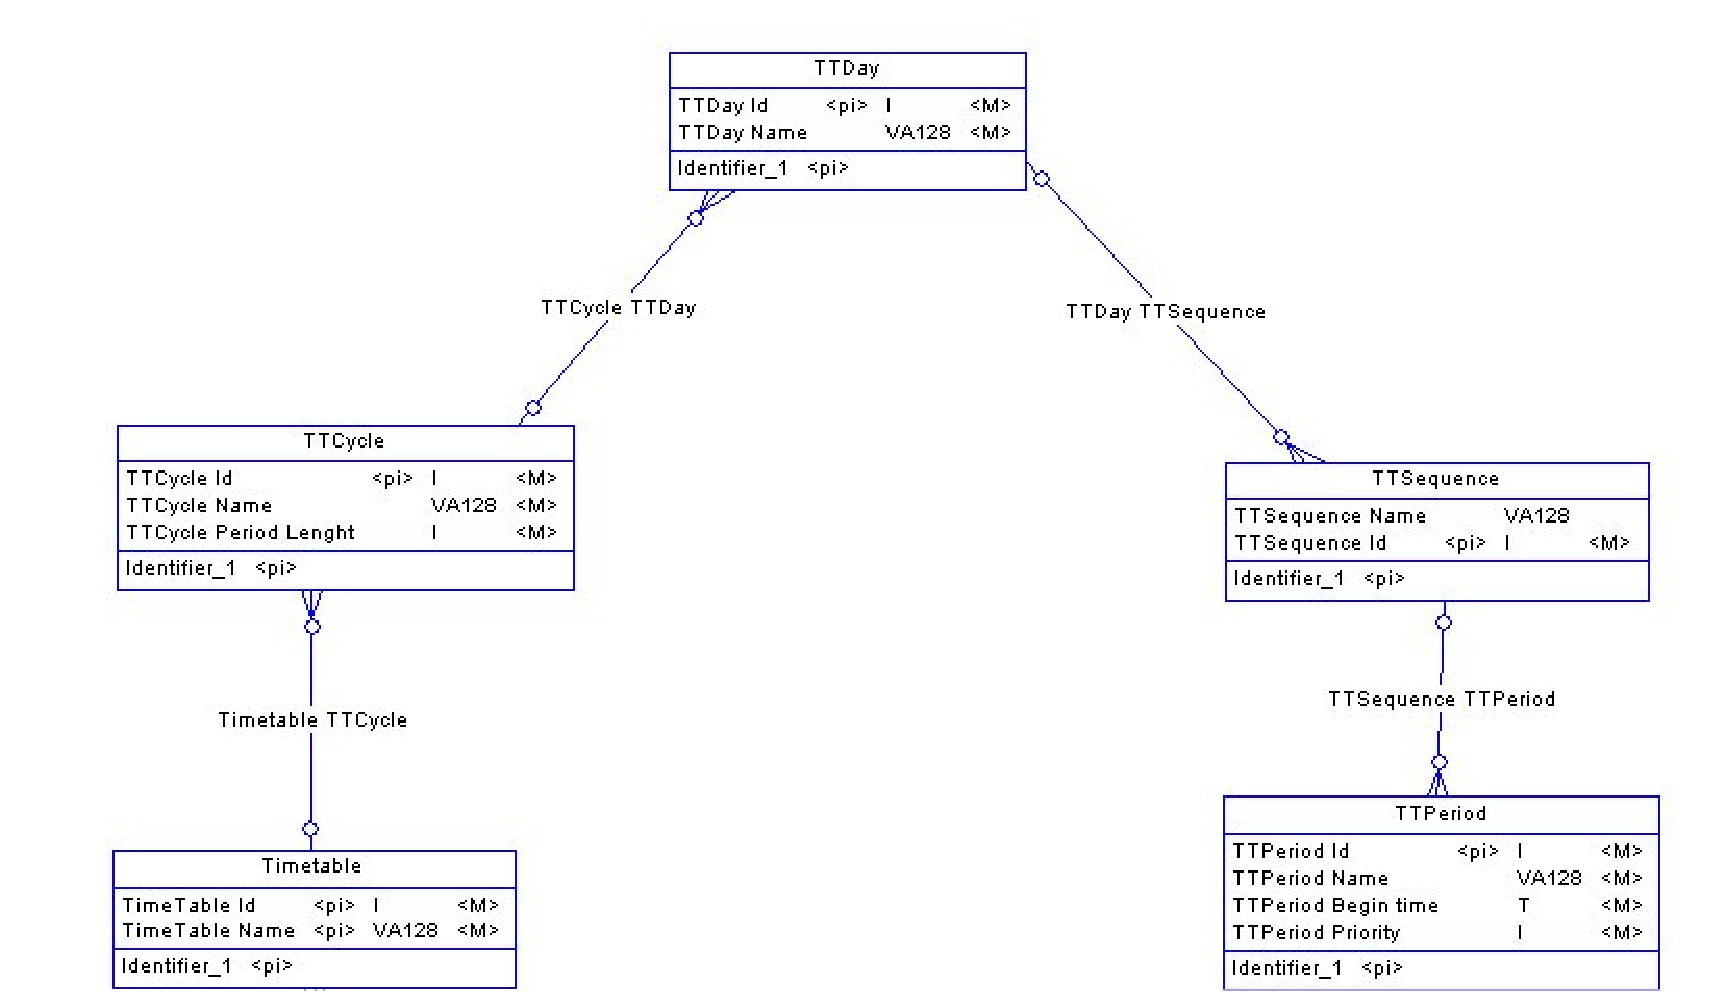
\includegraphics[width=300pt]{SDD/images/ttstruct.eps}
    \caption{Description de la grille horaire}\label{struct}
  \end{center}
\end{figure*}


\subsubsection{Description du sous-composant optimization}

Le sous-composant optimization comporte l'ensemble des �v�nements,
ainsi que les diff�rents algorithmes (organis�s autour du pattern
strat�gie).
\begin{description}
    \item[Ensemble des �v�nements: ] l'ensemble des �v�nements est
    une structure contruite � partir de la structure composite
    SetOfxxx. Dans cette structure le composite est repr�sent� par
    l'entit� \verb!SetOfEvents! et la feuille repr�sent� par
    l'entit� \verb!EventAttach!.
    \item[Pattern strat�gie: ] il permet de d�finir une famille
    d'algorithmes, les encapsules et les rend interchangeables.
    L'impl�mentation de ce pattern se fera de sorte � repr�senter
    le contexte par l'entit� \verb!TestConditions!, la strat�gie
    par l'entit� \verb!Algorithm! et les strat�gies concr�tes par
    les entit�s \verb!TestxxxConditions!.
    \item[Algorithme d'affectation initiale: ] il permet ...
    \item[Algorithme de mixage de groupes d'�tudiants: ] il permet
    ...
    \item[Algorithme de construction d'horaire: ] il permet ...
    \item[Algorithme d'affectation de locaux: ] il permet ...
\end{description}


\subsection{Description de la vue}

\diamant{} est une application avec une interface utilisateur
graphique (GUI). Elle utilise une interface principale comme point
d'entr�e (fen�tre principale - \emph{main display}-
\verb!DApplication!). L'interface principale int�gre trois
composants: la barre de menu (\verb!DMenuBar!), le m�diateur
(\verb!DMediator!) et la barre d'outils (\verb!DToolBar!).

\begin{figure*}[h]
  % Requires \usepackage{graphicx}
  \begin{center}
    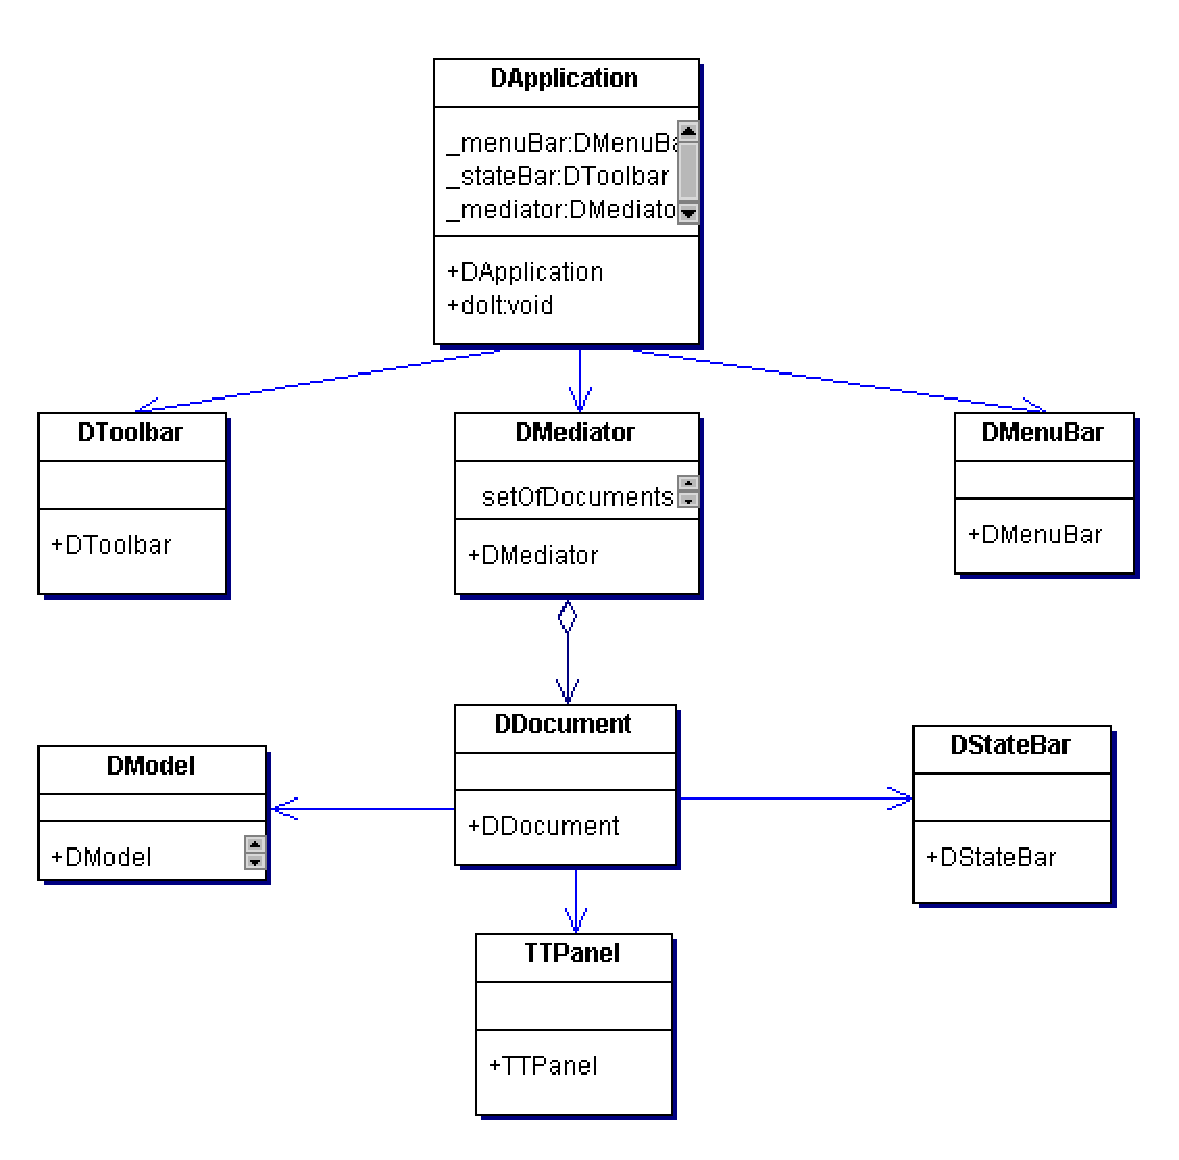
\includegraphics[width=300pt]{SDD/images/application.eps}
    \caption{Description des associations � partir du point d'entr�e}\label{application}
  \end{center}
\end{figure*}

\subsubsection{Barre de menu}

La barre de menu permet d'ex�cuter des commandes (traitements,
lancement de dialogues) en cliquant sur le menu associ�. Sa structure
s'inspire du pattern de commande (voir figure \ref{command}) afin
d'encapsuler une requ�te dans un objet, nous permettant de param�trer
le client avec diff�rentes requ�tes.

\begin{figure*}[h]
  % Requires \usepackage{graphicx}
  \begin{center}
    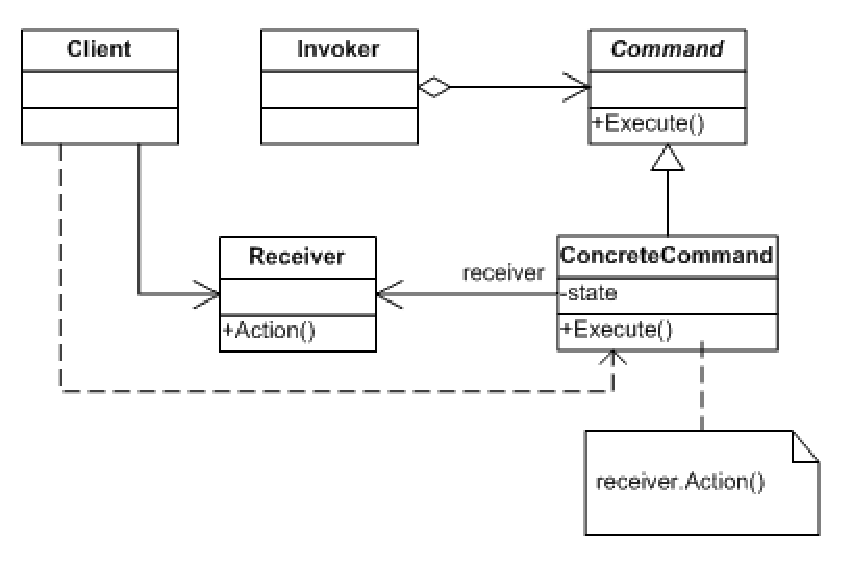
\includegraphics[width=250pt]{SDD/images/command.eps}
    \caption{Description du pattern de commande de la barre de
    menu}\label{command}
  \end{center}
\end{figure*}

Les principales classes et objets participants dans ce pattern
sont les suivantes:

\begin{description}
    \item[\verb!Command!: ] elle d�clare une interface permettant
    d'ex�cuter une op�ration. Elle gardera le m�me nom dans
    \diamant{}.
    \item[\verb!Invoker!: ] elle externalise la requ�te de la commande.
    Elle sera identifi�e dans \diamant{} par la classe CmdMenu.
    \item[\verb!ConcreteCommand!: ] elle impl�mente la m�thode Execute
    qui sera invoqu�e. Elle sera identifi�e dans \diamant{} par
    les classes de nom xxxCmd.
\end{description}

\subsubsection{Barre d'outils}

La barre d'outils facilite, acc�l�re et optimise la navigation
dans la grille horaire. Elle permet d'ajouter ou supprimer des
jours, modifier le nom d'une journ�e, modifier la priorit� d'une
ou de plusieurs p�riodes � la fois.

\subsubsection{M�diateur}

Le m�diateur est le corps de l'interface graphique, il est compos�
d'une collection de documents (\verb!DDocument!), ce qui lui
permet de g�rer plusieurs documents ou plusieurs horaires. Un
document (voir figure \ref{document}) est quant � lui compos�
d'une barre d'�tat (\verb!DStateBar!), d'un panneau de grille
horaire (\verb!TTPanel!) et d'un mod�le (\verb!DModel!).

\begin{figure*}[h]
  % Requires \usepackage{graphicx}
  \begin{center}
    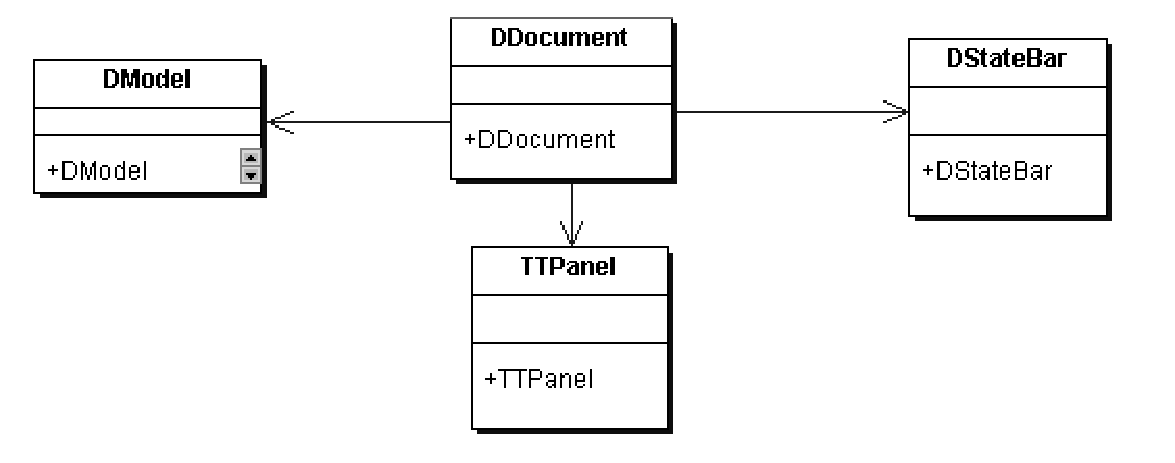
\includegraphics[width=250pt]{SDD/images/mediator.eps}
    \caption{Description d'un Document}\label{document}
  \end{center}
\end{figure*}

\begin{description}
    \item[Barre d'�tat: ] c'est la lisi�re situ�e au bas de la fen�tre et affichant des
    renseignements sur les enseignants, les locaux, les activit�s,
    les �tudiants, les �v�nements et les conflits.
    \item[Panneau de grille horaire: ] c'est la partie centrale de la
    fen�tre, elle pr�sente la grille horaire sous la forme d'un
    calendrier (jour, s�quence, p�riode) et indique pour chaque
    p�riode, le nombre d'�v�nements assign� et les conflits
    g�n�r�s dans cette p�riode.
    \item[Mod�le: ] il contient les donn�es sp�cifiques de \dx{}.
\end{description}

\subsection{Description du contr�leur}

\subsection{Probl�mes de conception}

\textcolor[rgb]{1.00,0.00,0.00}{L'architecture de \dx{} n'est pas
totalement conforme au mod�le MVC. En effet, certaines vues (exp:
\verb!dInterface.dAffectation.EditActivityDlg.ApplyChanges()!)
impl�mentent des m�thodes modifiant l'�tat du mod�le, ce qui cr�ait
une d�pendance bi-directionnelle entre le mod�le et la vue.} \corrpascal{on parle au pr�sent, puis au pass�.}

\section{D�composition des donn�es}

Les donn�es d'entr�e de \diamant{} sont de trois types: les
donn�es des ressources � partager (les enseignants, les locaux,
les activit�s et les �tudiants), la grille horaire
(\emph{timetable}) et les param�tres.

\subsection{Description des enseignants}

Voir section \ref{instructor}

\subsection{Description des locaux}

Voir section \ref{room}

\subsection{Description des activit�s}

Voir section \ref{activity}

\subsection{Description des �tudiants}

Voir section \ref{student}

\subsection{Description de la grille horaire}

\subsection{Description des pr�f�rences}

%\chapter{D�pendance}

Cette section d�crit les diff�rentes d�pendances d�crites aux sections \ref{module}, \ref{process} et \ref{data}

\section{D�pendances intermodule (Mod�le objet)}

\section{D�pendance interprocessus}

\section{D�pendance entre donn�es}

\section{D�pendance entre �tats}

\section{D�pendance entre couches} 
%\chapter{Description des interfaces}

Cette section d�crit les interfaces pour le mod�le objet.

\section{Interface de modules}
\subsection{Description module 1}
\subsection{Description module 2}

\section{Interface de processus}
\subsection{Description processus 1}
\subsection{Description processus 2}


\part{Conception d�taill�e}
\chapter{Conception d�taill�e}

\section{Conception d�taill� des modules}
\subsection{Module 1}
\subsection{Module 2}

\section{Conception d�taill� des Donn�es} 
\subsection{Type de donn�es 1}
\subsection{Type de donn�es 2}
\subsection{Type de donn�es 3} 



\appendix
%\chapter{Description des champs pour \diamant{} 1.5}\label{fields}

\begin{table}[h]
    \begin{tabular}{*{5}{|c}|} \hline
           \itshape Champ & \itshape �l�ment Diamant & \itshape  Description& \itshape Type \footnotemark[1] & \itshape Genre \footnotemark[2]\\ \hline
          Nom du local & Liste de locaux & - & A & \\ \cline{1-4}
          & Liste de locaux & - & A & \\ \cline{2-4}
          & Conflit de capa de locaux & Recalculer les conflits & C & \\ \cline{2-4}
          \raisebox{3.0ex}[1pt]{Capacit�} & P�riode & Rafra�chissement de la p�riode & C & \\ \cline{1-4}
          & Liste de locaux & - & A & \\ \cline{2-4}
          &  & V�rifier si les caract�ristiques & & \\
          &  & du local sont adapt�es & & \\
          \raisebox{4.5ex}[1pt]{Liste de} & \raisebox{3.0ex}[1pt]{Warning de locaux} & � la nature du cours & \raisebox{3.0ex}[1pt]{C} &  \\ \cline{2-4}
          \raisebox{4.5ex}[1pt]{caract�ristiques} & P�riode & Rafra�chissement de la p�riode & C & \raisebox{12.0ex}[1pt]{D} \\ \hline
    \end{tabular}
    \caption{\emph{Fichier de locaux} }
    \label{tableLocaux}
\end{table}
\footnotetext[1]{A: champs affect� - C: champs calcul�} \footnotetext[2]{S: champs statique (immuable) - D: champs dynamique (modifiable)}

\begin{table}[h]
    \begin{tabular}{*{5}{|c}|} \hline
          \itshape Champ & \itshape �l�ment Diamant & \itshape Description & \itshape Type \footnotemark[1] & \itshape Genre \footnotemark[2]\\ \hline
          Instructeur ID(nom) & Liste de professeurs & - & A & S \\ \hline
          & Liste de disp. de profs. & - & A & \\ \cline{2-4}
          & Conflit de disp. de profs. & Recalculer les conflits & C & \\ \cline{2-4}
          \raisebox{3.0ex}[1pt]{Disponibilit�} & P�riode & Rafra�chissement de p�riode & C & \raisebox{3.0ex}[1pt]{D} \\\hline
    \end{tabular}
    \caption{\emph{Fichier de Enseignants}}
    \label{tableEnseignants}
\end{table}

\begin{table}[h]
    \begin{tabular}{*{5}{|c}|} \hline
          \itshape Champ & \itshape �l�ment Diamant & \itshape Description & \itshape Type \footnotemark[1] & \itshape Genre \footnotemark[2]\\ \hline
          Matricule & & - & & S \\ \cline{1-1} \cline{3-3} \cline{5-5}
          Nom et pr�nom & & - & & S \\ \cline{1-1} \cline{3-3} \cline{5-5}
          Sexe & & - & & D \\ \cline{1-1} \cline{3-3} \cline{5-5}
          �tat & \raisebox{4.0ex}[1pt]{Liste d'�tudiants} & - & \raisebox{4.0ex}[1pt]{A} & D \\ \hline
          �tudiant.Activit�ID & & - & & \\ \cline{1-1} \cline{3-3}
          �tudiant.Activit�Nature & \raisebox{1.0ex}[1pt]{Conflits d'�tudiants et} & - & &  \\ \cline{1-1} \cline{3-3}
          �tudiant.Num�roGroupe & \raisebox{1.0ex}[1pt]{Conflits de capacit� de locaux} & - & \raisebox{3.0ex}[1pt]{C} & \raisebox{3.0ex}[1pt]{D} \\ \cline{1-1} \hline
    \end{tabular}
    \caption{\emph{Fichier d'�tudiants}}
    \label{tableEtudiants}
\end{table}


\begin{table}[h]
    \begin{tabular}{*{5}{|c}|} \hline
          \itshape Champ & \itshape �l�ment Diamant & \itshape Description & \itshape Type & \itshape Genre\\ \hline \hline
          Nom d'activit� & Liste d'activit�s & - & A & S \\ \hline
          & Liste d'activit�s & - & A & \\ \cline{2-4}
          & Conflits de locaux & Recalculer les conflits & & \\ \cline{2-2}
          & Conflits de disp. de profs. & si les activit�s sont d�j� & & \\ \cline{2-2}
          \raisebox{4.5ex}[1pt]{Include} & Conflit d'�tudiants & plac�es dans la grille & \raisebox{3.0ex}[1pt]{C} & \raisebox{4.5ex}[1pt]{D} \\ \hline
          Session & Liste d'activit�s & - & A & D \\ \hline
          & Liste de sous-activit�s & - & A & \\ \cline{2-4}
          & Liste d'activit�s & - & A & \\ \cline{2-4}
          & & Dans le cas o� il y a eu un & & \\
          & \raisebox{1.5ex}[1pt]{Warning de locaux} & changement de nature & \raisebox{1.5ex}[1pt]{C} & \\ \cline{2-4}
          & & Dans le cas o� il y a eu une & & \\
          \raisebox{7.0ex}[1pt]{Sous-Activit�.Nature} & \raisebox{1.5ex}[1pt]{Tous les conflits} & insertion/suppression de nature & \raisebox{1.5ex}[1pt]{C} & \raisebox{7.5ex}[1pt]{D} \\ \hline
          & Liste de groupes & - & & \\ \cline{2-3}
          & Liste de sous-activit�s & - & & \\ \cline{2-3}
          & Liste d'activit�s & - & \raisebox{3.0ex}[1pt]{A} &  \\ \cline{2-4}
          & & Dans le cas o� il y a eu une & & \\
          \raisebox{6.0ex}[1pt]{Groupe.Num�ro} & \raisebox{1.5ex}[1pt]{Tous les conflits} & suppression de groupe & \raisebox{1.5ex}[1pt]{C} & \raisebox{6.0ex}[1pt]{S} \\ \hline
          & Liste de bloques & - & & \\ \cline{2-3}
          & Liste de groupes & - & & \\ \cline{2-3}
          & Liste de sous-activit�s & - & & \\ \cline{2-3}
          & Liste d'activit�s & - & \raisebox{4.5ex}[1pt]{A} &  \\ \cline{2-4}
          & & Dans le cas o� il y a eu une & & \\
          \raisebox{6.0ex}[1pt]{Bloque.Num�ro} & \raisebox{1.5ex}[1pt]{Tous les conflits} & suppression de bloque & \raisebox{1.5ex}[1pt]{C} & \raisebox{7.5ex}[1pt]{S} \\ \hline
          & Toutes les listes & - & A & \\ \cline{2-4}
          & Conflit de locaux & - & C & \\ \cline{2-4}
          \raisebox{3.0ex}[1pt]{Bloque.LocalID} & Warning de locaux & - & C & \raisebox{3.0ex}[1pt]{D} \\ \hline
          & Toutes les listes & - & A & \\ \cline{2-4}
          \raisebox{1.5ex}[1pt]{Bloque.P�riodeID} & Tous les conflits & - & C & \raisebox{1.5ex}[1pt]{D} \\ \hline
          & Toutes les listes & - & A & \\ \cline{2-4}
          \raisebox{1.5ex}[1pt]{Bloque.Dure�} & Tous les conflits & - & C & \raisebox{1.5ex}[1pt]{D} \\ \hline
          & Toutes les listes & - & A & \\ \cline{2-4}
          \raisebox{1.5ex}[1pt]{Bloque.Activit�Type} & Warning de locaux & - & C & \raisebox{1.5ex}[1pt]{D} \\ \hline
          & Toutes les listes & - & A & \\ \cline{2-4}
          \raisebox{1.5ex}[1pt]{Bloque.Plac�} & Tous les conflits & - & C & \raisebox{1.5ex}[1pt]{D} \\ \hline
          & Toutes les listes & - & A & \\ \cline{2-4}
          \raisebox{1.5ex}[1pt]{Bloque.Fig�} & Tous les conflits & - & C & \raisebox{1.5ex}[1pt]{D} \\ \hline
          & Toutes les listes & - & A & \\ \cline{2-4}
          \raisebox{1.5ex}[1pt]{Bloque.Instructeur} & Conflit d'instructeur & - & C & \raisebox{1.5ex}[1pt]{D} \\ \hline
    \end{tabular}
    \caption{\emph{Fichier de Cours}}
    \label{tableCours}
\end{table}


  % after \\: \hline or \cline{col0-col2} \cline{col3-col4} .

%\chapter*{Glossaire}

Bla bla bla bla bla.

Bla bla bla bla bla.

%\chapter*{Index}

A
AAA
ABC.

B
Bla bla bla bla bla.

%\include{formules}
\end{articleDX}
\end{document}
